\documentclass[a4paper,12pt]{article} % добавить leqno в [] для нумерации слева
\usepackage[a4paper,top=1.3cm,bottom=2cm,left=1.5cm,right=1.5cm,marginparwidth=0.75cm]{geometry}
%%% Работа с русским языком
\usepackage{cmap}					% поиск в PDF
\usepackage[warn]{mathtext} 		% русские буквы в фомулах
\usepackage[T2A]{fontenc}			% кодировка
\usepackage[utf8]{inputenc}			% кодировка исходного текста
\usepackage[english,russian]{babel}	% локализация и переносы
\usepackage{physics}
\usepackage{multirow}
\usepackage{float}
\restylefloat{table}


\usepackage{graphicx}

\usepackage{wrapfig}
\usepackage{tabularx}

\usepackage{hyperref}
\usepackage[rgb]{xcolor}
\hypersetup{
	colorlinks=true,urlcolor=blue
}

%%% Дополнительная работа с математикой
\usepackage{amsmath,amsfonts,amssymb,amsthm,mathtools} % AMS
\usepackage{icomma} % "Умная" запятая: $0,2$ --- число, $0, 2$ --- перечисление

%% Номера формул
\mathtoolsset{showonlyrefs=true} % Показывать номера только у тех формул, на которые есть \eqref{} в тексте.

%% Шрифты
\usepackage{euscript}	 % Шрифт Евклид
\usepackage{mathrsfs} % Красивый матшрифт

%% Свои команды
\DeclareMathOperator{\sgn}{\mathop{sgn}}

%% Перенос знаков в формулах (по Львовскому)
\newcommand*{\hm}[1]{#1\nobreak\discretionary{}
	{\hbox{$\mathsurround=0pt #1$}}{}}

\date{\today}

\begin{document}

\begin{titlepage}
	\begin{center}
		{\large МОСКОВСКИЙ ФИЗИКО-ТЕХНИЧЕСКИЙ ИНСТИТУТ (НАЦИОНАЛЬНЫЙ ИССЛЕДОВАТЕЛЬСКИЙ УНИВЕРСИТЕТ)}
	\end{center}
	\begin{center}
		{\large Физтех-школа физики и исследований им. Ландау}
	\end{center}
	
	
	\vspace{4.5cm}
	{\huge
		\begin{center}
			{\bf Лабораторная работа 1.1.6}\\
				Изучение электронного осциллографа
		\end{center}
	}
	\vspace{2cm}
	\begin{flushright}
		{\LARGE Автор:\\ Третьяков Александр \\
			\vspace{0.2cm}
			Б02-206}
	\end{flushright}
	\vspace{8cm}
	\begin{center}
		Долгопрудный\\
		\today
	\end{center}
\end{titlepage}

\section{Введение}

\textbf{Цель работы:} ознакомление с устройством и работой осциллографа и изучение его основных характеристик.\\
\textbf{В работе используются:} осциллограф \textit{GWINSTEK GOS-620}, генераторы электрических сигналов, соединительные кабели.

\section{Теоретические сведения}

Осциллограф - регистрирующий прибор, в кагором исследуемое напряжение (сигнал) преобразуется в видимый на экране график изменения напряжения во времени. Осциллограф широко используется в физическом эксперименте. С его помощью можно исследовать изменение во времени любых физических величин, которые могут быть преобразованы в электрические сигналы.

\begin{wrapfigure}{r}{10cm}
	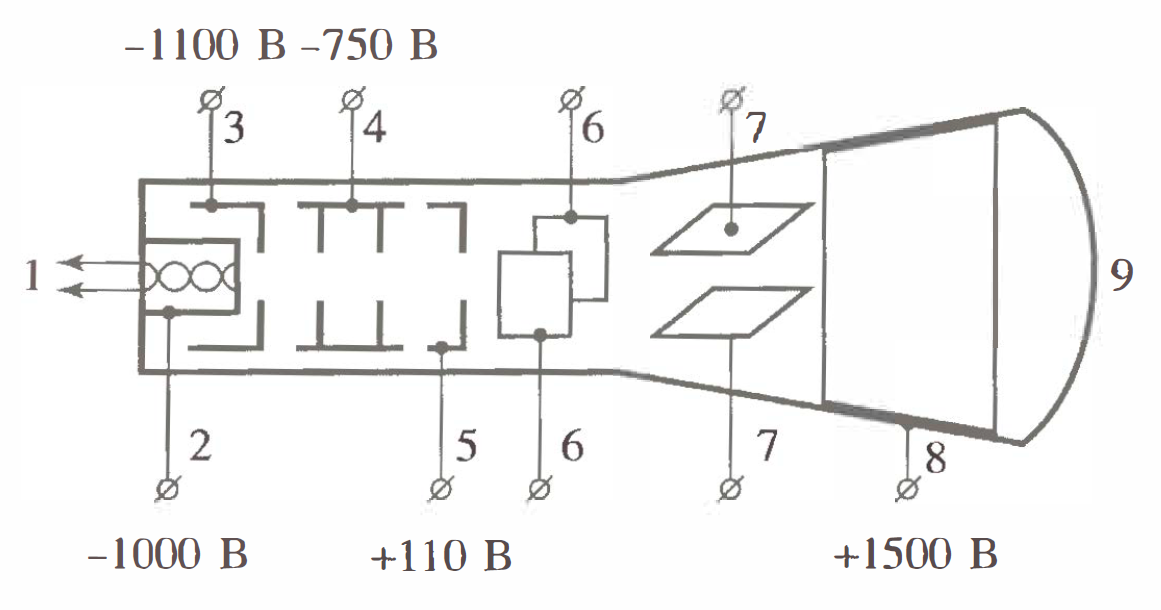
\includegraphics[width=10cm]{truba.png}
	\caption{Электронно-лучевая трубка}
	\label{ELT}
\end{wrapfigure}

На рис. \ref{ELT} показано устройство основной части электронного осциллографа -- электронно-лучевой трубки. Трубка представляет собой откачанную до высокого вакуума колбу, в кагорой расположены: подогреватель катода \textbf{1}, катод \textbf{2}, модулятор \textbf{3} (электрод, управляющий яркостью изображения), первый (фокусирующий) анод \textbf{4}, второй (ускоряющий) анод \textbf{5}, горизонтально и вертикально отклоняющие пластины \textbf{6} и \textbf{7}, третий (ускоряющий) анод \textbf{8}, экран \textbf{9}. 

При наблюдении периодических и особенно быстропротекающих процессов важно получить на экране осциллографа неподвижное изображение сигнала. Для этого нужно, чтобы период развертки был кратен периоду изучаемого сигнала. Однако, как правило, точное соотношение периодов соблюсти трудно из-за нестабильности генератора развертки или самого изучаемого процесса. Поэтому используют принудительное согласование периодов, при котором изучаемое напряжение «навязывает» свой период генератору развертки. При этом начало прямого хода развёртки должно совпадать строго с одной и той же характерной точкой исследуемого периодического сигнала. Процесс привязки начала развертки к характерным точкам сигнала называется \textit{синхронизацией} развертки с сигналом.

В процессе работы с осциллографом всегда следует учитывать частотные характеристики каналов вертикального и горизонтального отклонения: амплитудно-частотную характеристику (АЧХ) и фазо-­частотную характеристику (ФЧХ). Если на вход <<Y>> осциллографа подаётся синусоидальное напряжение $ U_y=U_0\sin\left(2\pi ft\right) $ амплитудой $ U_0 $ и частотой $ f $, то для перемещения луча на экране ЭЛТ можно записать: $ y=y_0\left(f\right)\sin\left(2\pi ft + \Delta\Phi_y\left(f\right)\right) $. Здесь $ U_0 $ -- амплитуда перемещения луча на частоте $ f $, $ \Delta\Phi_y\left(f\right) $ - разность между фазой колебаний перемещения луча $ y $ и фазой колебаний входного сигнала $ U_y $ на частоте $ f $ (сдвиг фаз).

Тогда АЧХ канала вертикального отклонения есть зависимость:

\begin{equation}
K_y\left(f\right) = \frac{y_0\left(f\right)}{U_0}, \label{ahch}
\end{equation}
а ФЧХ - зависимость $ \Delta\Phi_y\left(f\right) $.

При сложении двух взаимно перпендикулярных колебаний с равными или кратными частотами, поданных на входы осциллографа, луч описывает на экране неподвижные замкнутые кривые, которые называются \textbf{фигурами Лиссажу}. При небольшом нарушении кратности частот форма фигур медленно меняется, а при большом - картина размывается.

Фигура, которую описывает луч при сложении колебаний, имеющих одинаковую частоту, представляет собой эллипс. Ориентация этого эллипса зависит от разности фаз колебаний $ \left(\varphi_2-\varphi_1\right) $.

\begin{wrapfigure}{r}{10cm}
	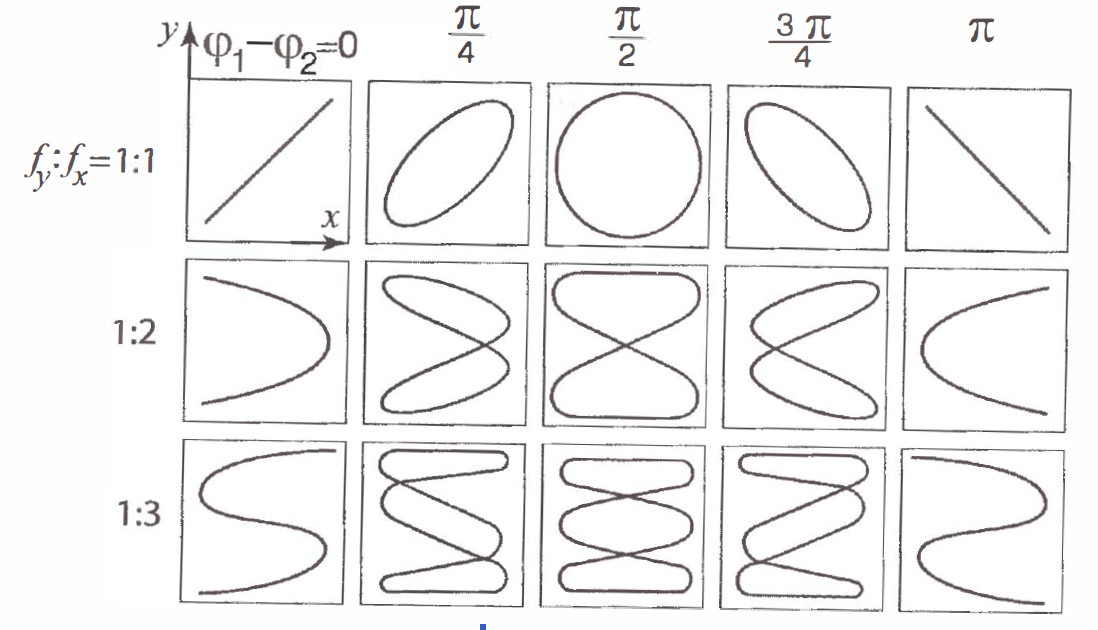
\includegraphics[width=10cm]{l_prim.png}
	\caption{Фигуры Лиссажу для колебаний одинаковой амплитуды}
	\label{l_prim}
\end{wrapfigure}

В общем случае вид фигуры Лиссажу зависит от соотношений между периодами (частотами), фазами и амплитудами складываемых колебаний. Некоторые частные случаи фигур Лиссажу для разных периодов и фаз показаны на рис. \ref{l_prim}. Зная параметры одного колебания, 
например $ f_x $, можно по фигуре Лиссажу определить параметры другого колебания -- $ f_y $. На полученное изображение накладывают мысленно две линии -- горизонтальную и вертикальную, не проходящие через узлы фигуры. Фиксируют число пересечений с горизонтальной линией $ n_x $ и вертикальной линией $ n_y $ . Отношение частот $ f_y/f_x $ равно отношению $ n_x/n_y $. 

\section{Ход работы}

\subsection{Наблюдение периодического сигнала от генератора и измерение его частоты}

Получим на экране осциллографа устойчивую картину периодического (синусоидального) сигнала, подаваемого с генератора, и с помощью горизонтальной шкалы экрана осциллографа проведём измерение периода и частоты сигнала. Полученные результаты занесём в таблицу \ref{tab:chastota}.

%\begin{table}[H]
%	\centering
%	\begin{tabular}{|c|c|c|c|c|c|c|c|c|c|}
%		\hline
%		№ & $ f_\text{ЗГ} $, Гц & $ T' $, дел & TIME/DIV, мс & $ T $, мс & $ \delta T $, мс & $ \varepsilon_T $, \% & $ f_\text{изм} $, Гц & $ \delta f $, Гц & $ \left| f_\text{ЗГ} - f_\text{изм} \right| $, Гц \\ \hline
%		1 & 998 & 5 & 0,2 & 1,00 & 0,02 & 2 & 1000 & 20 & 2 \\ \hline
%		2 & 3030 & 6,8 & 0,05 & 0,34 & 0,005 & 1 & 2941 & 43 & 89 \\ \hline
%		3 & 5500 & 9,2 & 0,02 & 0,18 & 0,002 & 1 & 5435 & 59 & 65 \\ \hline
%		4 & 10030 & 5 & 0,02 & 0,10 & 0,002 & 2 & 10000 & 200 & 30 \\ \hline
%		5 & 503,7 & 4 & 0,5 & 2,00 & 0,05 & 3 & 500 & 13 & 4 \\ \hline
%	\end{tabular}
%	\caption{Определение частоты сигнала при помощи осциллографа}
%	\label{tab:chastota}
%\end{table}

Погрешность прямого измерения периода сигнала $ \delta T $ равна половине цены малого деления осциллографа, т.е. $ \frac{1}{10} $ части от TIME/DIV.

Частоту сигнала можно вычислить по следующей формуле:

\begin{equation}
f_\text{изм} = \frac{1}{T}.
\end{equation}

Тогда погрешность вычисления $ f_\text{изм} $ равна:

\begin{equation}
\delta f_\text{изм} = f_\text{изм}\varepsilon_T.
\end{equation}
Полученные данные заносим в таблицу \ref{tab:chastota}.

\subsection{Измерение амплитуды сигнала}

С помощью вертикальной шкалы осциллографа проведём измерение амплитуды сигнала. Для этого установим значение частоты входного сигнала осциллографа 1 кГц, затем измерим отношение $ \frac{U_max}{U_min} $, которые способен выдавать генератор. Результаты измерений занесем  таблицу \ref{tab:my-table}

%\begin{table}[H]
%	\centering
%	\begin{tabular}{|c|c|c|c|c|c|c|c|c|}
%		\hline
%		$ U_{max} $, В & $ \delta U_{max} $, В & $ \varepsilon_{U_{max}} $, \% & $ U_{min} $, В & $ \delta U_{min} $, В & $ \varepsilon_{U_{min}} $, \% & $ \beta $, дБ & $ \delta\beta $, дБ & $ \varepsilon_\beta $, \% \\ \hline
%		21 & 0,5 & 2,3 & 0,013 & 0,0005 & 3,8 & 64,2 & 0,4 & 0,6 \\ \hline
%	\end{tabular}
%	\caption{Измерение амплитуды сигнала}
%	\label{tab:my-table}
%\end{table}

Выразим отношение максимального и минимального уровней сигнала в
децибелах [дБ]. Децибел — логарифмическая единица ослабления или
усиления, определяемая по формуле:

\begin{equation}
\beta_{21} \left[\text{дБ}\right]=10\lg\frac{P_1}{P_2}=20\lg\frac{U_1}{U_2}.
\end{equation}

Тогда

\begin{equation}
\beta = 20 \lg \frac{U_{max}}{U_{min}} = 64,2 \text{ дБ}.
\end{equation}
Погрешность вычисления $ \beta $ можно вычислить по формуле:

\begin{equation}
\delta \beta = \sqrt{\left(\frac{20\varepsilon_{U_{max}}}{\ln 10}\right)^2+\left(\frac{20\varepsilon_{U_{min}}}{\ln 10}\right)^2} = 0,4 \text{ дБ}.
\end{equation}

Итого получаем:
\begin{itemize}
	\item \underline{$ \beta = \left(64,2 \pm 0,4\right) $ дБ, $ \left(\varepsilon = 0,6 \%\right) $}
\end{itemize}

\subsection{Измерение амплитудно-частотной характеристики осциллографа}

Амплитудо-частотной характеристикой (АЧХ) измерительного прибора называют зависимость амплитуды измеряемого
сигнала от частоты сигнала, подаваемого на вход. Проведём измерение АЧХ используемого в работе осциллографа во всём диапазоне
рабочих частот генератора по формуле \eqref{ahch}.

Результаты измерений занесём в таблицу \ref{tab:ahch}.

%\begin{table}[H]
%	\centering
%	\begin{tabular}{|c|c|c|c|c|c|c|}
%		\hline
%		№ & 1 & 2 & 3 & 4 & 5 & 6 \\ \hline
%		$ f $, Гц & 1000 & 1 & 2 & $ 16\cdot10^6 $ & $ 23\cdot10^6 $ & $ 30\cdot10^6 $ \\ \hline
%		$ \lg f $ & 3 & 0 & 0,3 & 7,2 & 7,4 & 7,5 \\ \hline
%		$ 2U_{AC} $, дел & 5 & 1,4 & 2,6 & 4,6 & 3,8 & 3 \\ \hline
%		$ K_{AC} = \frac{U_{AC}}{U_0} $ & 1 & 0,28 & 0,52 & 0,92 & 0,76 & 0,6 \\ \hline
%		$ 2U_{DC} $, дел & 5 & 5 & 5 & 4,6 & 3,8 & 3 \\ \hline
%		$ K_{DC} = \frac{U_{DC}}{U_0} $ & 1 & 1 & 1 & 0,92 & 0,76 & 0,6 \\ \hline \hline
%		№ & 7 & 8 & 9 & 10 & 11 & 12 \\ \hline
%		$ f $, Гц & 10 & 50 & 200 & 2000 & 5000 & $ 20 \cdot 10^3 $ \\ \hline
%		$ \lg f $ & 1 & 1,7 & 2,3 & 3,3 & 3,7 & 4,3 \\ \hline
%		$ 2U_{AC} $, дел & 4,8 & 5 & 5 & 5 & 5 & 5 \\ \hline
%		$ K_{AC} = \frac{U_{AC}}{U_0} $ & 0,96 & 1 & 1 & 1 & 1 & 1 \\ \hline
%		$ 2U_{DC} $, дел & 5 & 5 & 5 & 5 & 5 & 5 \\ \hline
%		$ K_{DC} = \frac{U_{DC}}{U_0} $ & 1 & 1 & 1 & 1 & 1 & 1 \\ \hline
%	\end{tabular}
%	\caption{Измерение АХЧ осциллографа}
%	\label{tab:ahch}
%\end{table}
График зависимости АХЧ от частоты сигнала представлен на рис. \ref{ahch_graph}.

%\begin{figure}[H]
%	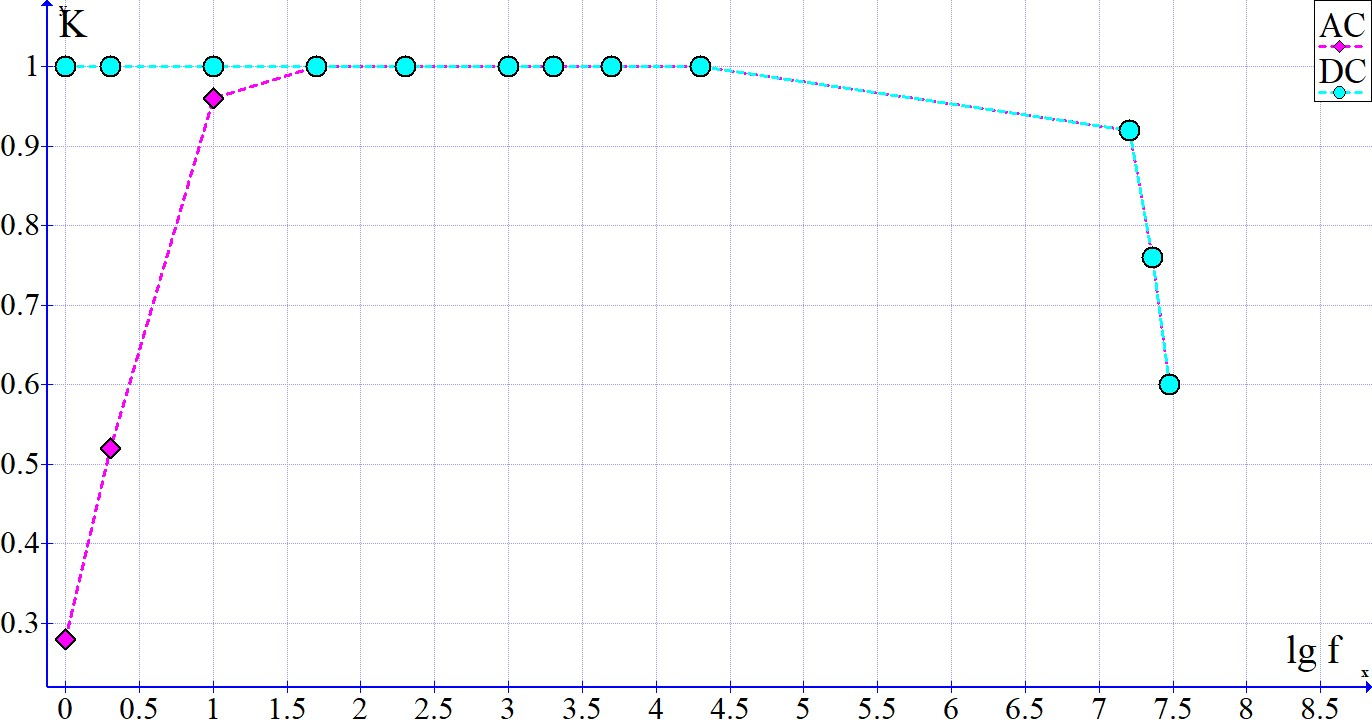
\includegraphics[scale=0.388]{ahch_graph.jpg}
%	\caption{График зависимости АХЧ от частоты сигнала}
%	\label{ahch_graph}
%\end{figure}

Причиной различия АХЧ осциллографа в разных режимах работы является ёмкость, включающаяся в схему осциллографа в режиме AC. При больших частотах её влияние становится мало, и оно почти не влияет на показания прибора, но на маленьких частотах оно становится значительным и способным изменить показания прибора.

\subsection{Измерение разности ФЧХ каналов осциллографа}

Фазо-частотной характеристикой (ФЧХ) называют зависимость разности
фаз входного и выходного сигналов от частоты.
Выключим внутреннюю развертку осциллографа, переведя переключатель
TIME/DIV в положение X–Y. В этом режиме отклонение луча на экране
пропорционально подаваемым на каналы напряжениям $ Y\left(t\right)= k_yU_y\left(t\right) $,
$ X\left(t\right) = k_xU_x\left(t\right) $ , где коэффициенты масштаба $ k_x, k_y $ определяются
положениями ручек VOLTS/DIV. Изменяя частоту генератора $ f $ во всем
доступном диапазоне, найдём участки, на которых изображение на экране
переходит из отрезка в невырожденный эллипс. На этих участках проведём
подробное измерение разности фаз $ \Delta \varphi\left(f\right) $ между каналами $ X $ и $ Y $ в
зависимости от частоты. Внесём измерения в таблицу \ref{tab:fchkh}.

%\begin{table}[H]
%	\centering
%	\begin{tabular}{|c|c|c|c|c|c|c|c|}
%		\hline
%		№ & 1 & 2 & 3 & 4 & 5 & 6 & 7 \\ \hline
%		$ f $, кГц & 600 & 1000 & 1200 & 1600 & 2300 & 2900 & 3500 \\ \hline
%		$ \lg f $ & 5,77 & 6 & 6,08 & 6,21 & 6,36 & 6,46 & 6,54 \\ \hline
%		сторона наклона & $ \nearrow $ & $ \nearrow $ & $ \nearrow $ & $ \nearrow $ & $ \circ $ & $ \nwarrow $ & $ \nwarrow $ \\ \hline
%		$ \left|2y_0\right| $, дел & 1,8 & 3,2 & 3,8 & 4,8 & 6 & 4,2 & 2 \\ \hline
%		$ \left|2A_y\right| $, дел & 6 & 6 & 6 & 6 & 6 & 6 & 6 \\ \hline
%		$ \arcsin\left|\frac{y_0}{A_y}\right| $, рад & 0,31 & 0,56 & 0,69 & 0,92 & 1,57 & 0,78 & 0,34 \\ \hline
%		$ \left|\Delta\varphi\right| $, рад & 0,31 & 0,56 & 0,69 & 0,92 & 1,57 & 2,37 & 2,81 \\ \hline \hline
%		№ & 8 & 9 & 10 & 11 & 12 & 13 & 14 \\ \hline
%		$ f $, кГц & 800 & 1500 & 1700 & 1900 & 2500 & 3000 & 3200 \\ \hline
%		$ \lg f $ & 5,91 & 6,18 & 6,23 & 6,28 & 6,39 & 6,48 & 6,51 \\ \hline
%		сторона наклона & $ \nearrow $ & $ \nearrow $ & $ \nearrow $ & $ \nearrow $ & $ \nwarrow $ & $ \nwarrow $ & $ \nwarrow $ \\ \hline
%		$ \left|2y_0\right| $, дел & 2,4 & 4,2 & 5 & 5,2 & 5,8 & 5,2 & 4,8 \\ \hline
%		$ \left|2A_y\right| $, дел & 6 & 6 & 6 & 6 & 6 & 6 & 6 \\ \hline
%		$ \arcsin\left|\frac{y_0}{A_y}\right| $, рад & 0,41 & 0,78 & 0,93 & 1,02 & 1,25 & 1,02 & 0,93 \\ \hline
%		$ \left|\Delta\varphi\right| $, рад & 0,41 & 0,76 & 0,93 & 1,02 & 1,89 & 2,52 & 2,65 \\ \hline
%	\end{tabular}
%	\caption{Зависимость разности фаз от частоты сигнала}
%	\label{tab:fchkh}
%\end{table}

\begin{wrapfigure}{r}{6cm}
	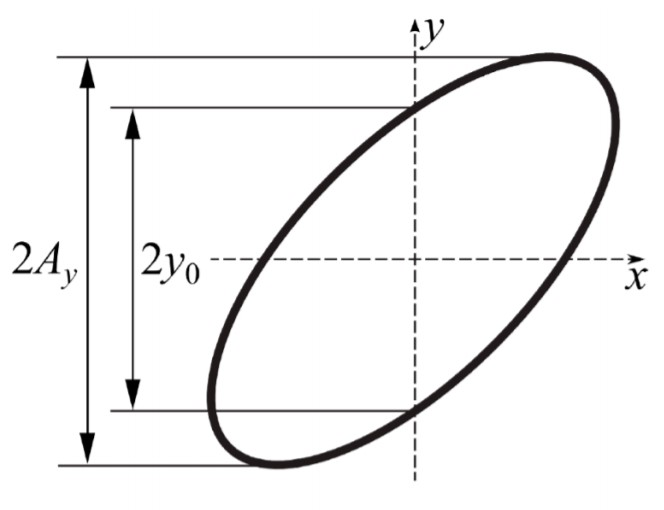
\includegraphics[width=6cm]{ellipse.jpg}
	\caption{К определению ФЧХ}
	\label{ellipse}
\end{wrapfigure}

При подаче на взаимно перпендикулярные отклоняющие пластины двух
синусоидальных сигналов траектория луча на экране осциллографа
представляет собой эллипс и может быть в общем виде описана
уравнениями

\begin{equation}
x\left(t\right) = A_x \sin\left(\omega t + \varphi_x\right),\text{ }y\left(t\right) = A_y \sin\left(\omega t + \varphi_y\right).
\end{equation}

Разность фаз $ \Delta \varphi = \varphi_y - \varphi_x $ можно выразить, получив:

\begin{equation}
\sin \left|\Delta \varphi\right| = \left|\frac{y_0}{A_y}\right|,
\end{equation}

где $ y_0 $ -- отклонение луча по вертикали в момент, когда его абсцисса
равна нулю; $ A_y $ -- амплитуда колебаний по оси $ y $ (см. рис. \ref{ellipse}).

Тогда
возможные значения модуля разности фаз:

\begin{equation}
\left|\Delta \varphi\right|=\arcsin\left|\frac{y_0}{A_y}\right|, \label{vpravo}
\end{equation}
или
\begin{equation}
\left|\Delta \varphi\right|=\pi - \arcsin\left|\frac{y_0}{A_y}\right|. \label{vlevo}
\end{equation}

При этом, если эллипс наклонён вправо (как на рис. \ref{ellipse}), то угол $ \Delta \varphi $ лежит в
интервале $ \left[-\frac{\pi}{2};\frac{\pi}{2}\right] $ -- имеет место формула \eqref{vpravo}; если эллипс наклонён влево, то $ \Delta \varphi \in \left[-\pi;-\frac{\pi}{2}\right]\cup\left[\frac{\pi}{2};\pi \right] $ -- необходимо использовать формулу \eqref{vlevo}.

По полученным данным можно построить график. Он представлен на рисунке \ref{raz_faz_graph}.

%\begin{figure}[H]
%	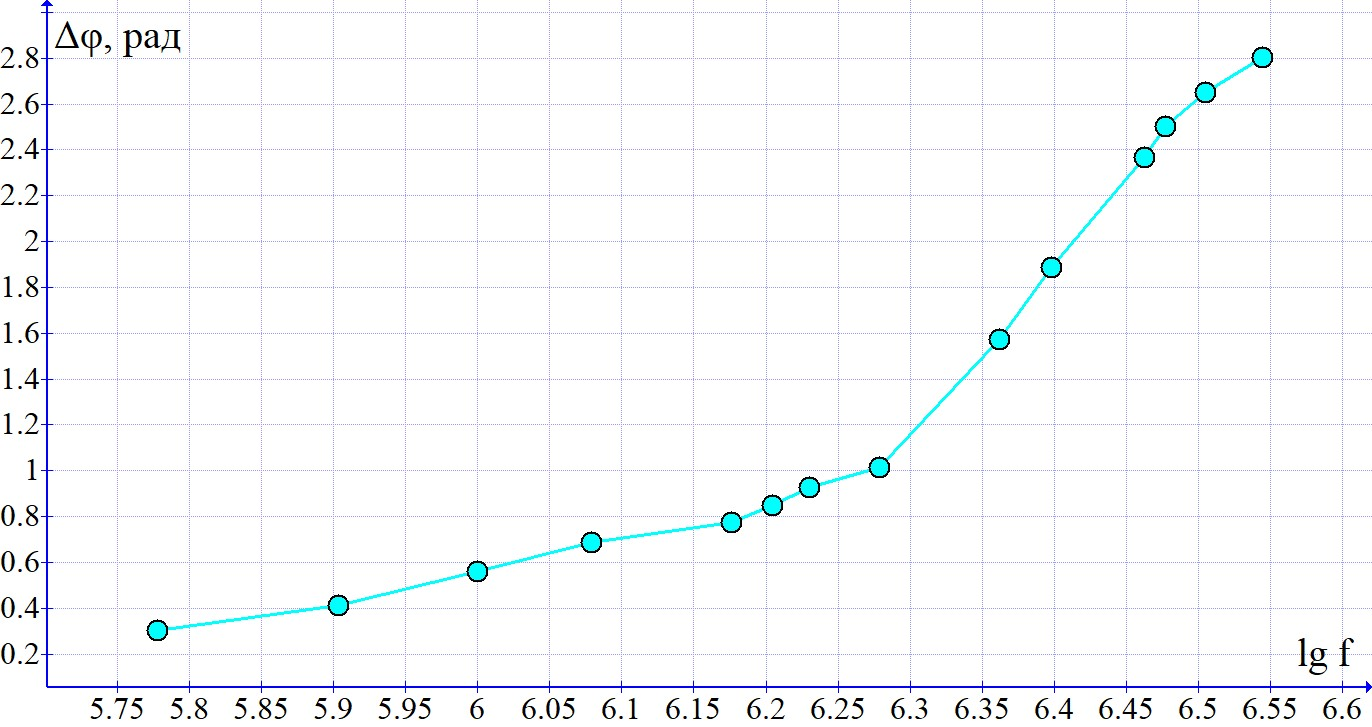
\includegraphics[scale=0.388]{raz_faz.jpg}
%	\caption{График зависимости разности фаз от частоты сигнала}
%	\label{raz_faz_graph}
%\end{figure}

\subsection{Наблюдение фигур Лиссажу}

Для наблюдения фигур Лиссажу необходимо подать на 2 входа осциллографа 2 	сигнала различной частоты, причём их частоты должны соотноситься, как целые числа. После получения устойчивой картины фигуры Лиссажу, с помощью изображения можно определить соотношение частот входных сигналов. Для определения соотношения необходимо провести 2 произвольные линии, параллельные осям и не пересекающие фигуру в узловых точках, затем посчитать колличество точек пересечения данных прямых с фигурой. Отношение этих чисел -- есть искомое соотношение между частотами. Фигуры Лиссажу для различных частот входных сигналов представлены на рисунке \ref{tab:lissazhu}.

\begin{table}[H]
	\centering
	\begin{tabular}{|c|c|}
		\hline
		{\Large $ \frac{f_y\strut }{f_x\strut } = \frac{1}{1}$}	& {\Large $ \frac{f_y\strut }{f_x\strut } = \frac{1}{2}$} \\ \hline
		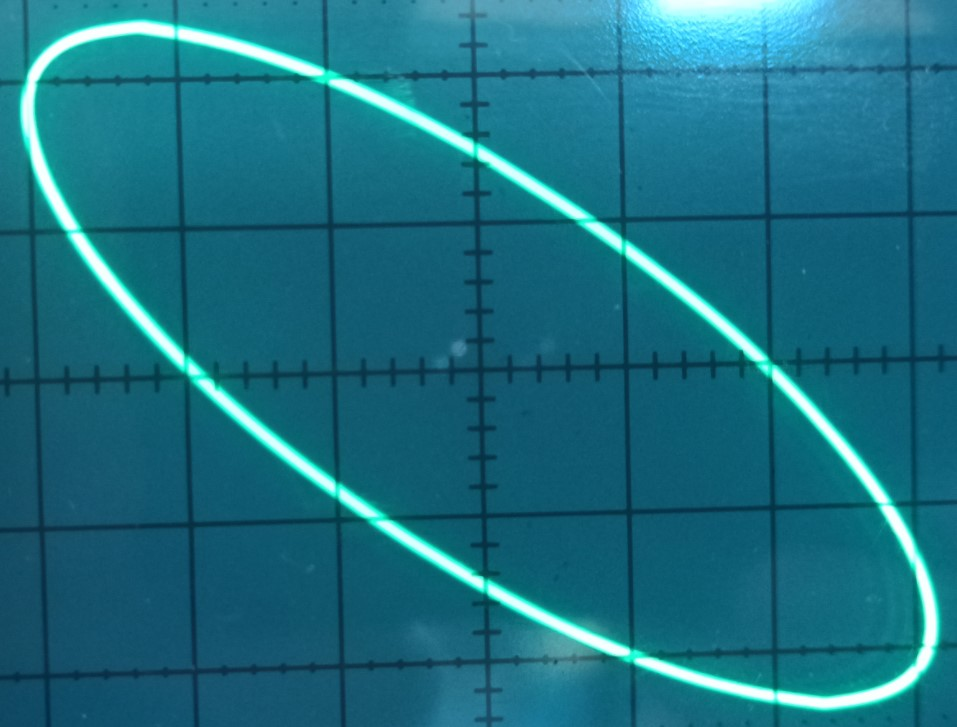
\includegraphics[width=0.5\textwidth]{liss_1_1.jpg}	& 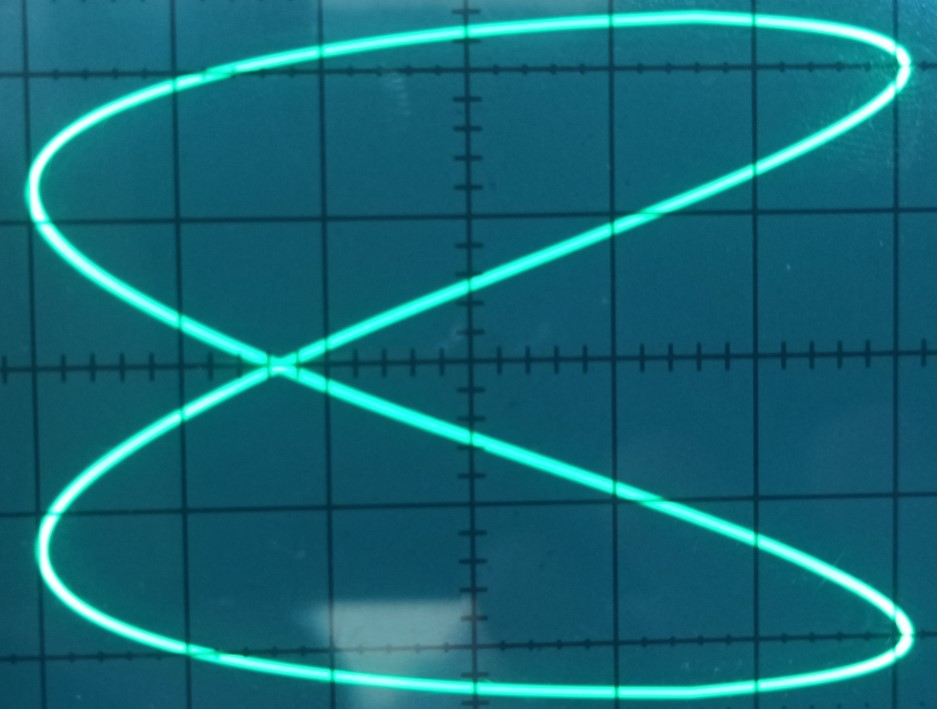
\includegraphics[width=0.5\textwidth]{liss_1_2.jpg}  \\ \hline
	\end{tabular}
\end{table}

\begin{table}[H]
	\centering
	\begin{tabular}{|c|c|}
		\hline
	{\Large $ \frac{f_y\strut }{f_x\strut } = \frac{1}{3}$}	& {\Large $ \frac{f_y\strut }{f_x\strut } = \frac{2}{3}$} \\ \hline
	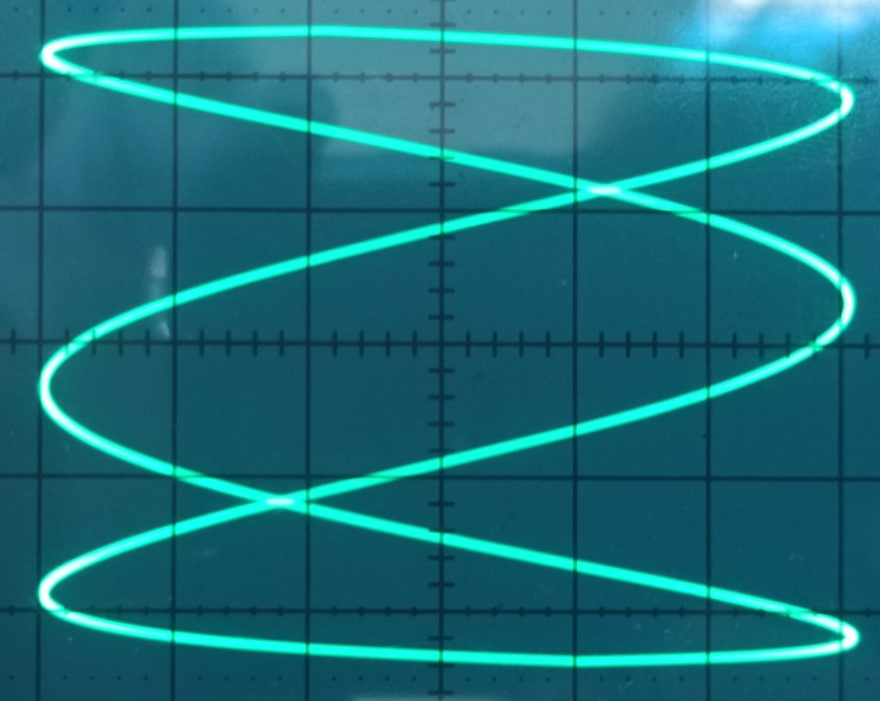
\includegraphics[width=0.5\textwidth]{liss_1_3.jpg}	& 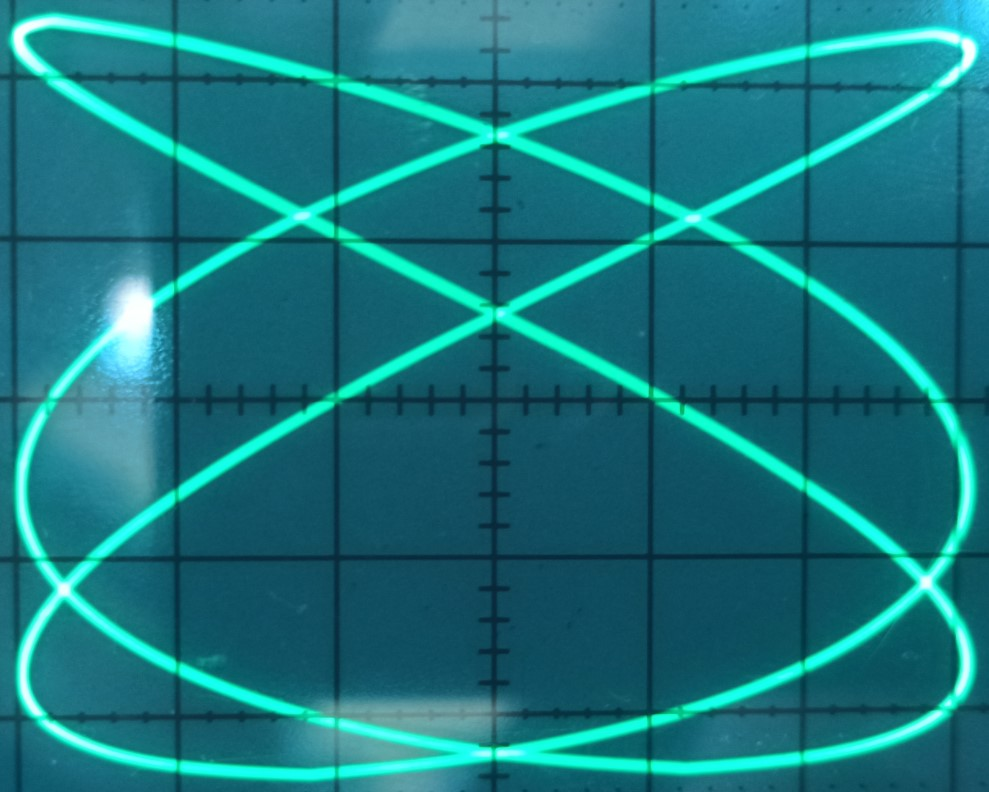
\includegraphics[width=0.5\textwidth]{liss_2_3.jpg} \\ \hline
	\end{tabular}
	\caption{Фигуры Лиссажу для различных частот входных сигналов}
	\label{tab:lissazhu}
\end{table}

\section{Обсуждение результатов и выводы}

\begin{itemize}
	\item Во время работы было изучено устройство осциллографа и принципы работы с ним
	\item При помощи осциллографа был исследован периодический сигнал и был определён его период и частота (максимальная погрешность измерений -- 3\%)
	\item Была измерена максимальная и минимальная амплитуда сигнала, которую может выдать генератор
	\item Для данного осциллографа была изучена зависимость АЧХ от частоты входного сигнала
	\item Было проведено измерение разности фазо-частотных характеристик каналов осциллографа
	\item При помощи осциллографа были получены изображения фигур Лиссажу. На практике были подтверждены методы определения соотношения между частотами сигналов, образующих фигуры Лиссажу
\end{itemize}




\end{document}